\documentclass{beamer}

\usepackage{cite}
\usepackage{amsmath,amssymb,amsfonts}
\usepackage{algorithmic}
\usepackage{graphicx}
\usepackage{textcomp}
\usepackage{xcolor}
\usepackage{array}
\usepackage{xmpmulti}
\usepackage{multirow}
\usepackage{bigstrut}
\usepackage{bigdelim}
\usepackage{hhline}
\usepackage{diagbox}
\usepackage{circuitikz}
\usepackage{comment}
\usepackage{multirow}
\usepackage{amsmath}
\usepackage{amssymb}
\usepackage{mathtools}
%\usepackage{movie15}
\usepackage{tkz-graph}
\usepackage{graphicx}
\usepackage{media9}
\usepackage{multimedia}
\usepackage{booktabs}
\usepackage{tkz-graph}
\usepackage{url}
\usepackage{comment}
\usepackage{bigstrut}
\usepackage{bigdelim}
\usepackage{hhline}
\usepackage{diagbox}
\usepackage{tikz}
\usepackage{xcolor,colortbl} % <---
\usepackage{lipsum}

\usepackage{tabularx}
\usepackage{wrapfig,lipsum,booktabs}

\usepackage{xcolor,colortbl}
\definecolor{gray}{rgb}{0.1,0.1,0.1}
\definecolor{light-gray1}{gray}{0.1}
%\definecolor{light-gray2}{cyan}{0.6}

\definecolor{light-gray2}{rgb}{0.9,0.9,0.9}



%\newcommand{\done}{\cellcolor{gray}}  %{0.9}
%\newcommand{\done}{\cellcolor{light-gray}}
%\newcommand{\done}{\cellcolor{gray}}
%\newcommand{\hcyan}[1]{{\color{teal} #1}}



%\newcommand{\done}{\cellcolor{light-gray1}}
\newcommand{\done}{\cellcolor{light-gray2}}




\usepackage{subfig}
%\usepackage{graphicx} % Allows including images
\usepackage{booktabs} % Allows the use of \toprule, \midrule and
%\bottomrule in tables
\usepackage{multimedia}


%\setbeamertemplate{footline}[text line]{} % makes the footer EMPTY


                         
                         
\usepackage{comment}
\usepackage{amsmath,amssymb}
\DeclareMathOperator{\E}{\mathbb{E}}
\usepackage{mathtools}
\usepackage{tikz}
\usepackage{nth}
\usepackage{setspace}
\usepackage{graphicx} 
\usepackage{caption}
\usepackage{mwe}
\setstretch{1.3}
\usepackage{mwe}
\setstretch{1.3}

%\usepackage[table]{xcolor}
%\usepackage{boldline} 

%\usepackage{tabularray}\%usepackage{xcolor}


\setlength{\arrayrulewidth}{0.01pt}

\DeclareRobustCommand{\rchi}{{\mathpalette\irchi\relax}}
\newcommand{\irchi}[2]{\raisebox{\depth}{$#1\chi$}}
\DeclarePairedDelimiterX{\norm}[1]{\lVert}{\rVert}{#1}


\usepackage{array,booktabs,arydshln,xcolor}
\newcommand\VRule[1][\arrayrulewidth]{\vrule width #1}


\mode<presentation> {

% The Beamer class comes with a number of default slide themes
% which change the colors and layouts of slides. Below this is a list
% of all the themes, uncomment each in turn to see what they look like.
%\usepackage{hyperref}
%\usetheme{default}
%\usetheme{AnnArbor}
%\usetheme{Antibes}
%\usetheme{Bergen}
%\usetheme{Berkeley}
%\usetheme{Berlin}
%\usetheme{Boadilla}
\usetheme{CambridgeUS}
%\usetheme{Copenhagen}
%\usetheme{Darmstadt}
%\usetheme{Dresden}
%\usetheme{Frankfurt}
%\usetheme{Goettingen}
%\usetheme{Hannover}
%\usetheme{Ilmenau}
%\usetheme{JuanLesPins}
%\usetheme{Luebeck}
%\usetheme{Madrid}
%\usetheme{Malmoe}
%\usetheme{Marburg}
%\usetheme{Montpellier}
%\usetheme{PaloAlto}
%\usetheme{Pittsburgh}
%\usetheme{Rochester}
%\usetheme{Singapore}
%\usetheme{Szeged}
%\usetheme{Warsaw}

% As well as themes, the Beamer class has a number of color themes
% for any slide theme. Uncomment each of these in turn to see how it
% changes the colors of your current slide theme.

%\usecolortheme{albatross}
%\usecolortheme{beaver}
%\usecolortheme{beetle}
%\usecolortheme{crane}
%\usecolortheme{dolphin}
%\usecolortheme{dove}
%\usecolortheme{fly}
%\usecolortheme{lily}
%\usecolortheme{orchid}
%\usecolortheme{rose}
%\usecolortheme{seagull}
%\usecolortheme{seahorse}
%\usecolortheme{whale}
%\usecolortheme{wolverine}

%\setbeamertemplate{footline} % To remove the footer line in all slides uncomment this line
%\setbeamertemplate{footline}[page number] % To replace the footer line in all slides with a simple slide count uncomment this line

%\setbeamertemplate{navigation symbols}{} % To remove the navigation symbols from the bottom of all slides uncomment this line
}

\makeatletter
% create the shape
\pgfcircdeclarebipole{}{\ctikzvalof{bipoles/interr/height 2}}{spst}{\ctikzvalof{bipoles/interr/height}}{\ctikzvalof{bipoles/interr/width}}{

    \pgfsetlinewidth{\pgfkeysvalueof{/tikz/circuitikz/bipoles/thickness}\pgfstartlinewidth}

    \pgfpathmoveto{\pgfpoint{\pgf@circ@res@left}{0pt}}
    \pgfpathlineto{\pgfpoint{.6\pgf@circ@res@right}{\pgf@circ@res@up}}
    \pgfusepath{draw}   
}


\def\pgf@circ@spst@path#1{\pgf@circ@bipole@path{spst}{#1}}
\tikzset{switch/.style = {\circuitikzbasekey, /tikz/to path=\pgf@circ@spst@path, l=#1}}
\tikzset{spst/.style = {switch = #1}}
\makeatother

\usepackage{graphicx} % Allows including images
\usepackage{booktabs} % Allows the use of \toprule, \midrule and \bottomrule in tables

\newcommand{\supersc}[1]{\texorpdfstring{\textsuperscript{#1}}{}}



\title[Tadipatri Uday Kiran Reddy]{ADCs for Direct RF Sampling}
\author{Tadipatri Uday Kiran Reddy - EE19BTECH11038}
\institute[]{IIT Hyderabad}
\date{\today}

\begin{document}
\begin{frame}
  \titlepage
\end{frame}

\begin{frame}{Introduction}
\begin{figure}
	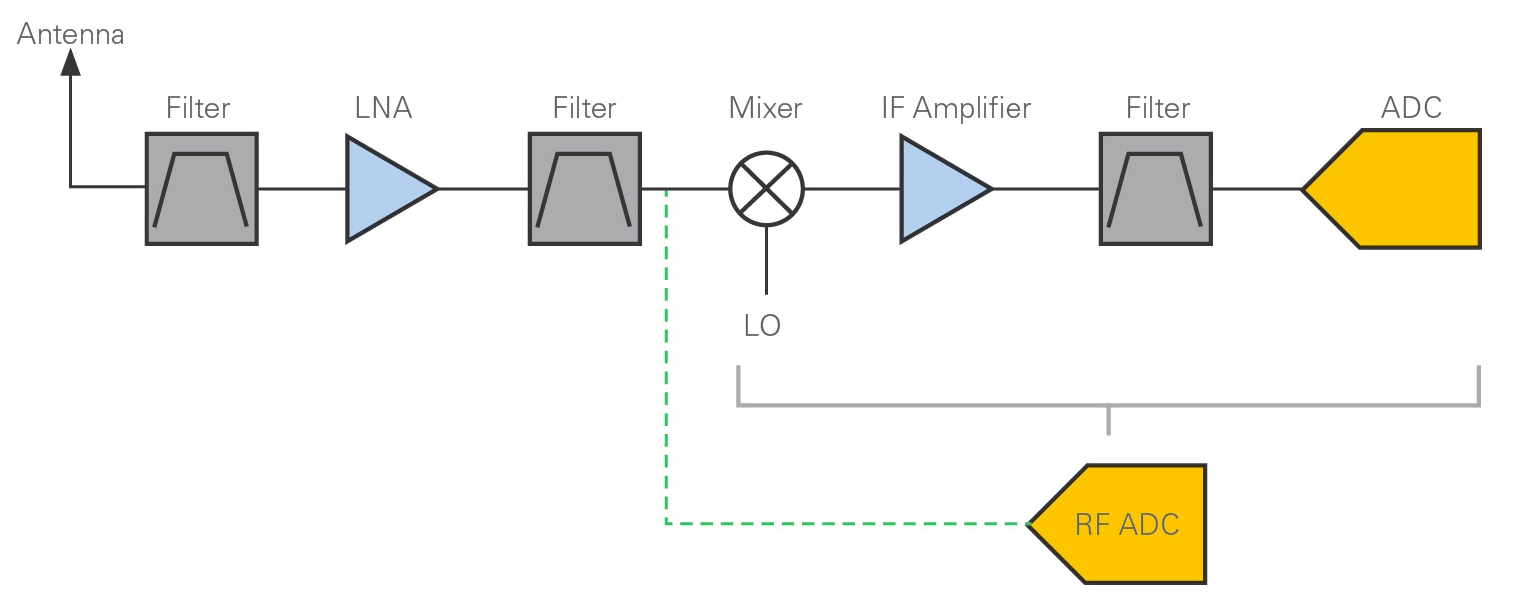
\includegraphics[scale=0.2]{./figs/arch.png}
\end{figure}
\pause
\begin{itemize}
	\item ADC architecture for sampling at RF with low power and area.
	\pause
	\item High sampling rate with relatively slow circuits, \textit{Time-Interleaved ADC}.
	\pause
	\item Minimize quantisation and noise error.
\end{itemize}

\end{frame}

\begin{frame}{Motivation for RF sampling}
\begin{figure}
	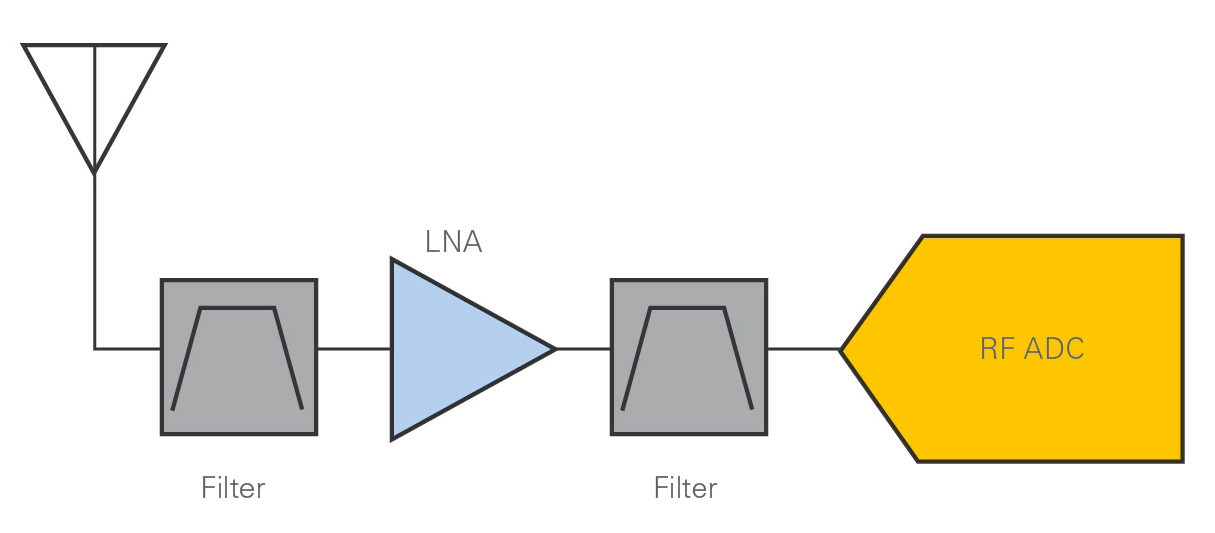
\includegraphics[scale=0.2]{./figs/rf_arch.png}
\end{figure}
\begin{itemize}
	\item Simpler hardware design due to elimination of analog frequency conversion.
	\pause
	\item Exploit the computing power of DSPs.
\end{itemize}
\end{frame}

\begin{frame}{Analog-to-Digital Converters}
	\begin{itemize}
		\item Sample the input signal at reconstructable rate and then Quantize.
		\pause
	\end{itemize}
	Types of converters,
	\pause
	\begin{itemize}
	\pause
		\item Nyquist-rate Converters, double the input bandwidth.
		\begin{equation*}
			SQNR = 6.02ENOB + 1.76 dB
		\end{equation*}
		\pause
		Noise spectral density is constant!
		\pause		
		\item Oversampled Converters, very high sampling rate, $OSR = \frac{f_s}{2f_B}$
		\begin{equation*}
			SQNR = 6.02ENOB + 1.76 + 10log(OSR)dB
		\end{equation*}
		\pause
		Noise spectral density at ROI is less!!
	\end{itemize}
\end{frame}

\begin{frame}{Limitations of S/H Circuit}
\begin{figure}[h]
\centering
\begin{circuitikz}[american]
\draw (0,-0.0) to[R,l=$R$] (2,-0.0);
\draw (2, 0.0) to [nos, l=$T_s$] (4, 0.0);
\draw (4,-0.0) to[C,l=$C$] (4,-2.0);
\draw (4,-2.0) node[ground]{};
\draw (4,-0.0) to[short, -o] (5,-0.0) node[label=$\hat{V}_{in}(nT_s)$]{};
\draw (0,-0.0) to[short, -o] (-1,-0.0) node[label=$V_{in}(t)$]{};
\end{circuitikz}
\pause
\begin{equation*}
	\frac{1}{RC} >> f_{in}
\end{equation*}
\pause
\begin{itemize}
	\item Difficult to construct S/H circuit with very high tracking BW.
	\pause
	\item Due to Low pass nature RF signal will attenuate.
\end{itemize}
\end{figure}
\end{frame}
\begin{frame}{Time-Interleaved ADC}
\begin{figure}
	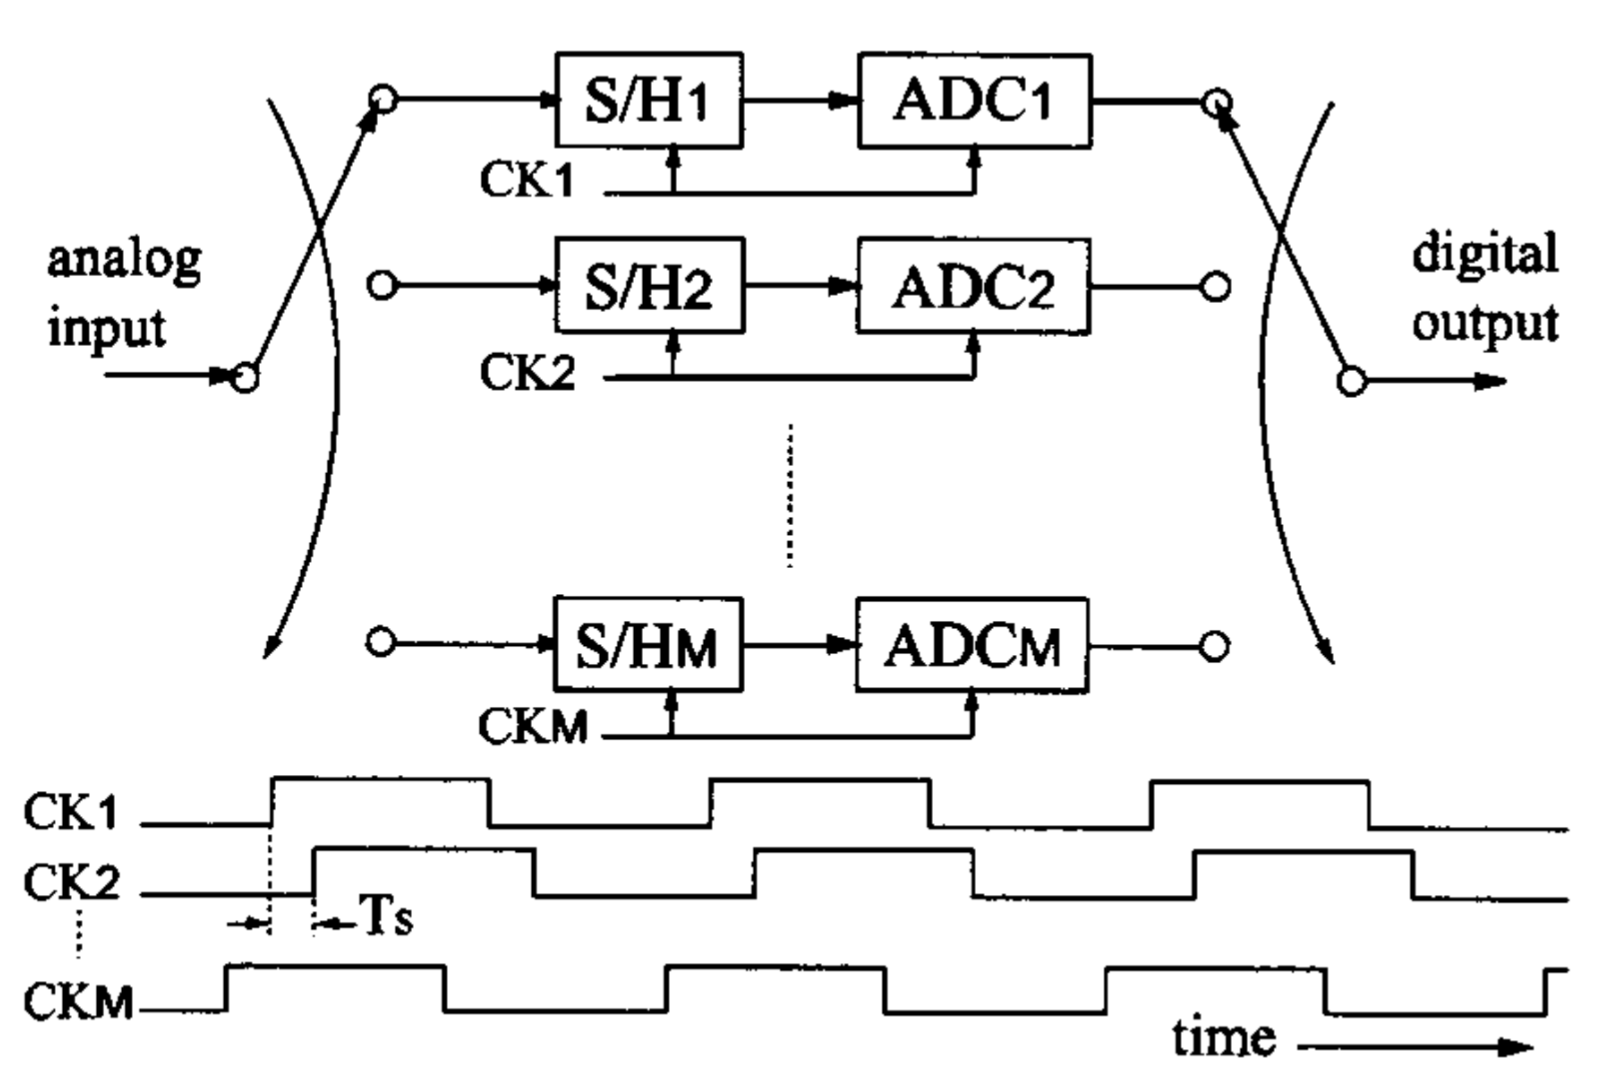
\includegraphics[scale=0.25]{./figs/tiadc.png}
\end{figure}
\pause
\begin{itemize}
	\item Required clock, $f_{clk} = f_s/M$
	\pause
	\item Phase difference, $\phi _i = \frac{2\pi(i-1)}{M}$
\end{itemize}
\end{frame}

\begin{frame}{Analysis of ADC based on VCO}
\begin{figure}
	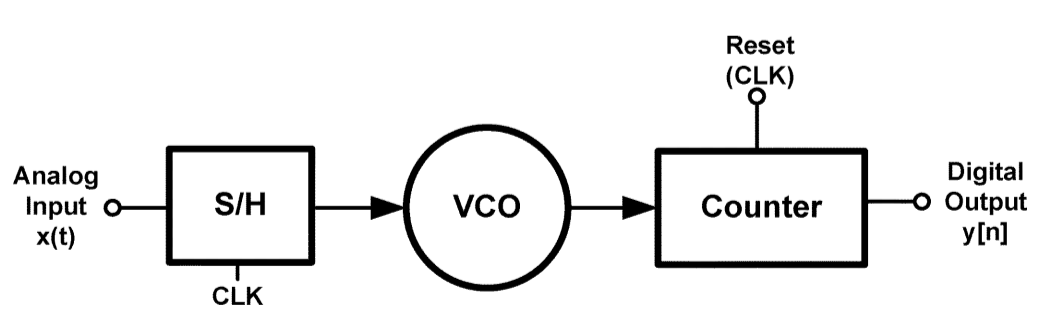
\includegraphics[scale=0.3]{./figs/Vco .png}
\end{figure}
\pause
\begin{itemize}
	\item VCO translates the input voltage to phase.
	\pause
	\item Counter, counts the number of rasing/falling edges.
\end{itemize}
\begin{gather*}
	\phi [n] = \int_{nT_s}^{(n+1)T_s}K_vx[n]dt + p_i[n] = G_vx[n] + e[n-1]
\end{gather*}
\end{frame}

\begin{frame}{Analysis of ADC based on VCO}
\begin{figure}
	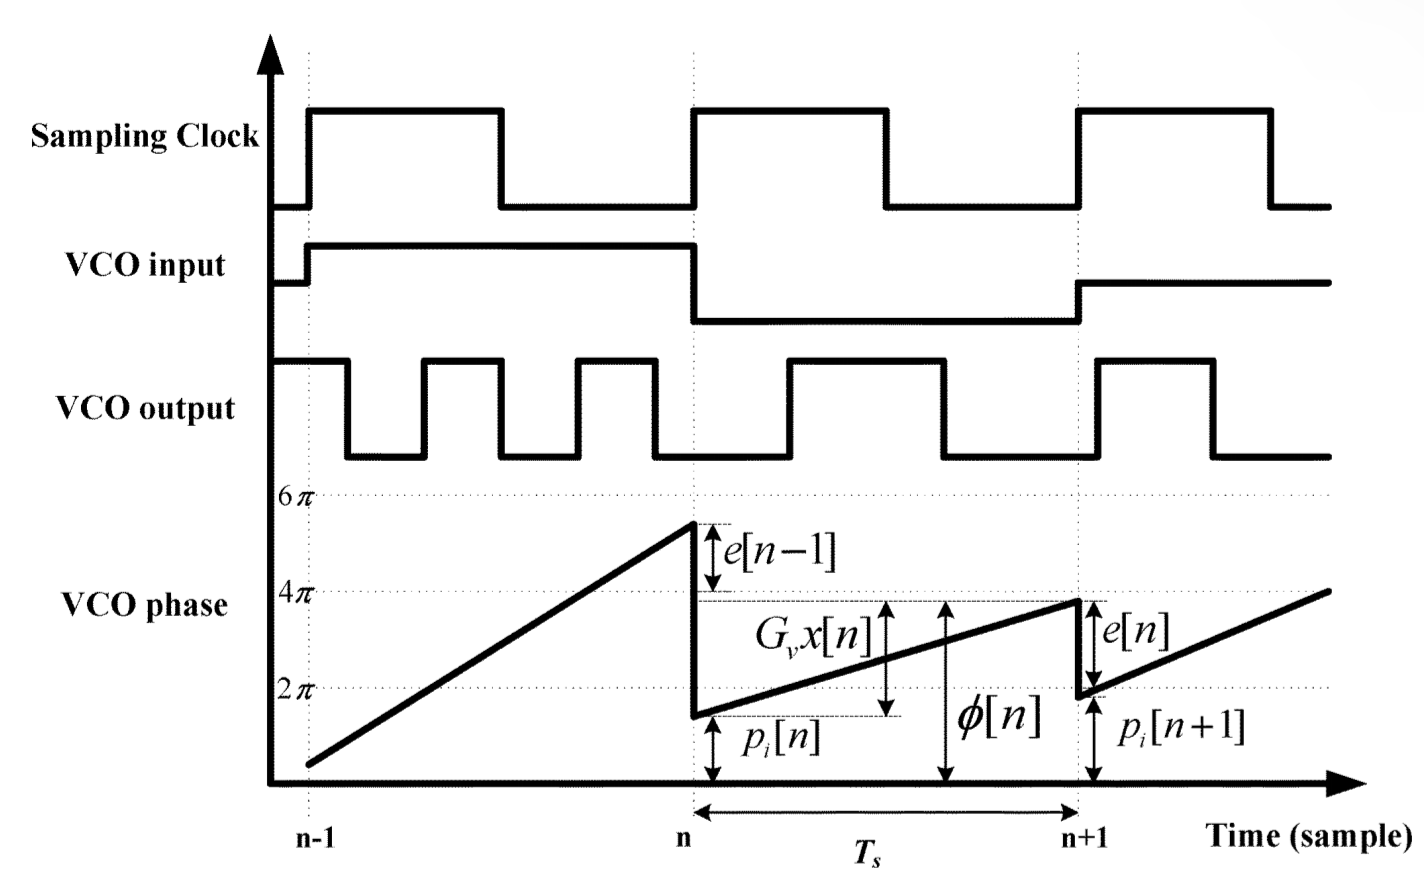
\includegraphics[scale=0.25]{./figs/Vcoplot.png}
\end{figure}
\vspace{-0.9cm}
\pause
\begin{gather*}
	y[n] = \frac{1}{2\pi}(\phi [n] - e[n]) = \frac{1}{2\pi}(G_vx[n] + e[n-1] - e[n])\\
	Y(z) = \frac{1}{2\pi}(G_vX(z) + (z^{-1} - 1)E(z))\\
	NTF(z) = \frac{1}{2\pi}(z^{-1} - 1) \implies |NTF(e^{j\omega})| = |2sin(\omega /2)|
\end{gather*}
\pause
\vspace{-1cm}
\begin{itemize}
	\item First order high-pass filter.
\end{itemize}
\end{frame}

\begin{frame}{Extension for N-th order ADC}
\vspace{-0.8cm}
\begin{gather*}
	NTF(z) = \frac{1}{2\pi}(z^{-N}-1)	
\end{gather*}
\vspace{-0.7cm}
\pause
\begin{itemize}
	\item Zeros will occur when $z = 1^{1/N} \implies \omega _k = \frac{2 \pi (k-1)}{N}$.
	\pause
	\item We will try to center our signal frequency at these zeros.
\end{itemize}
\pause
\begin{figure}
	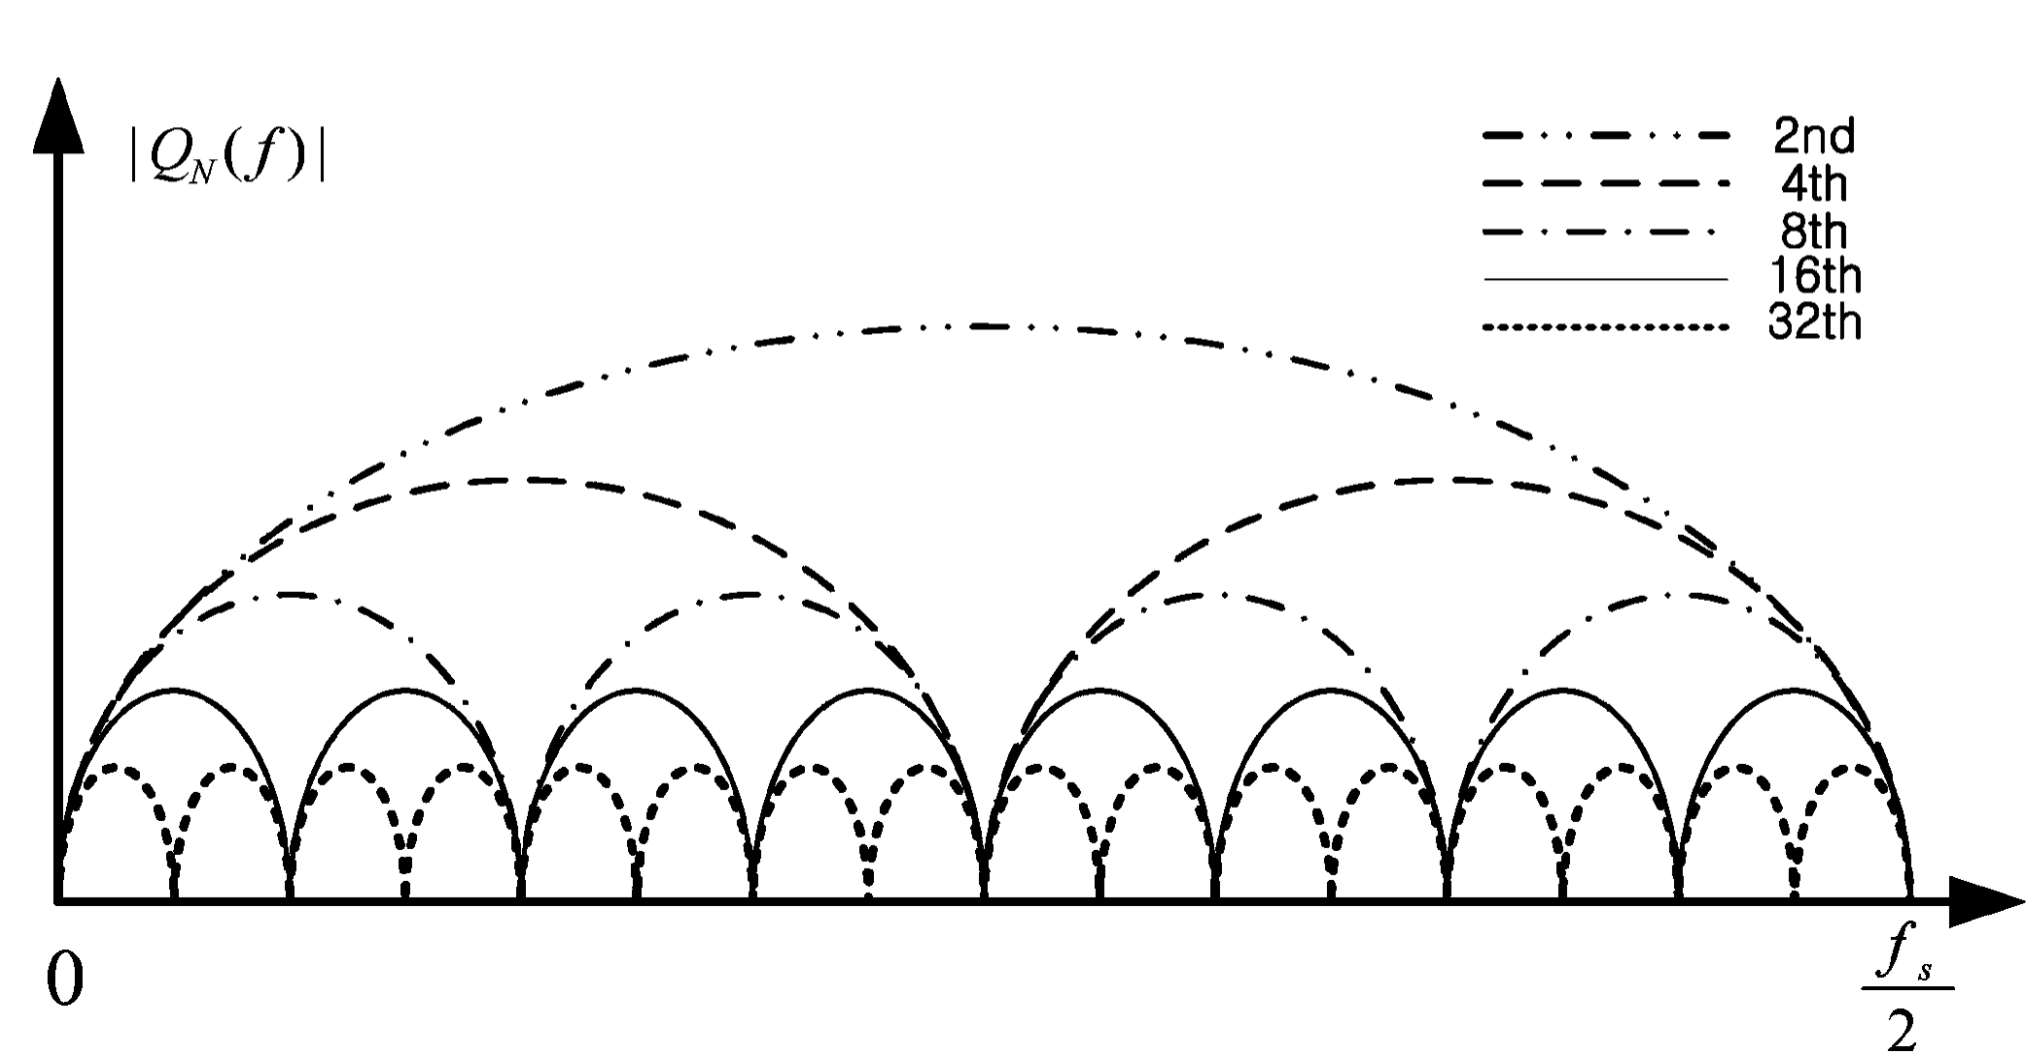
\includegraphics[scale=0.25]{./figs/Qorder.png}
\end{figure}
\end{frame}

\begin{frame}{Which Zero to center at?}
\begin{figure}
	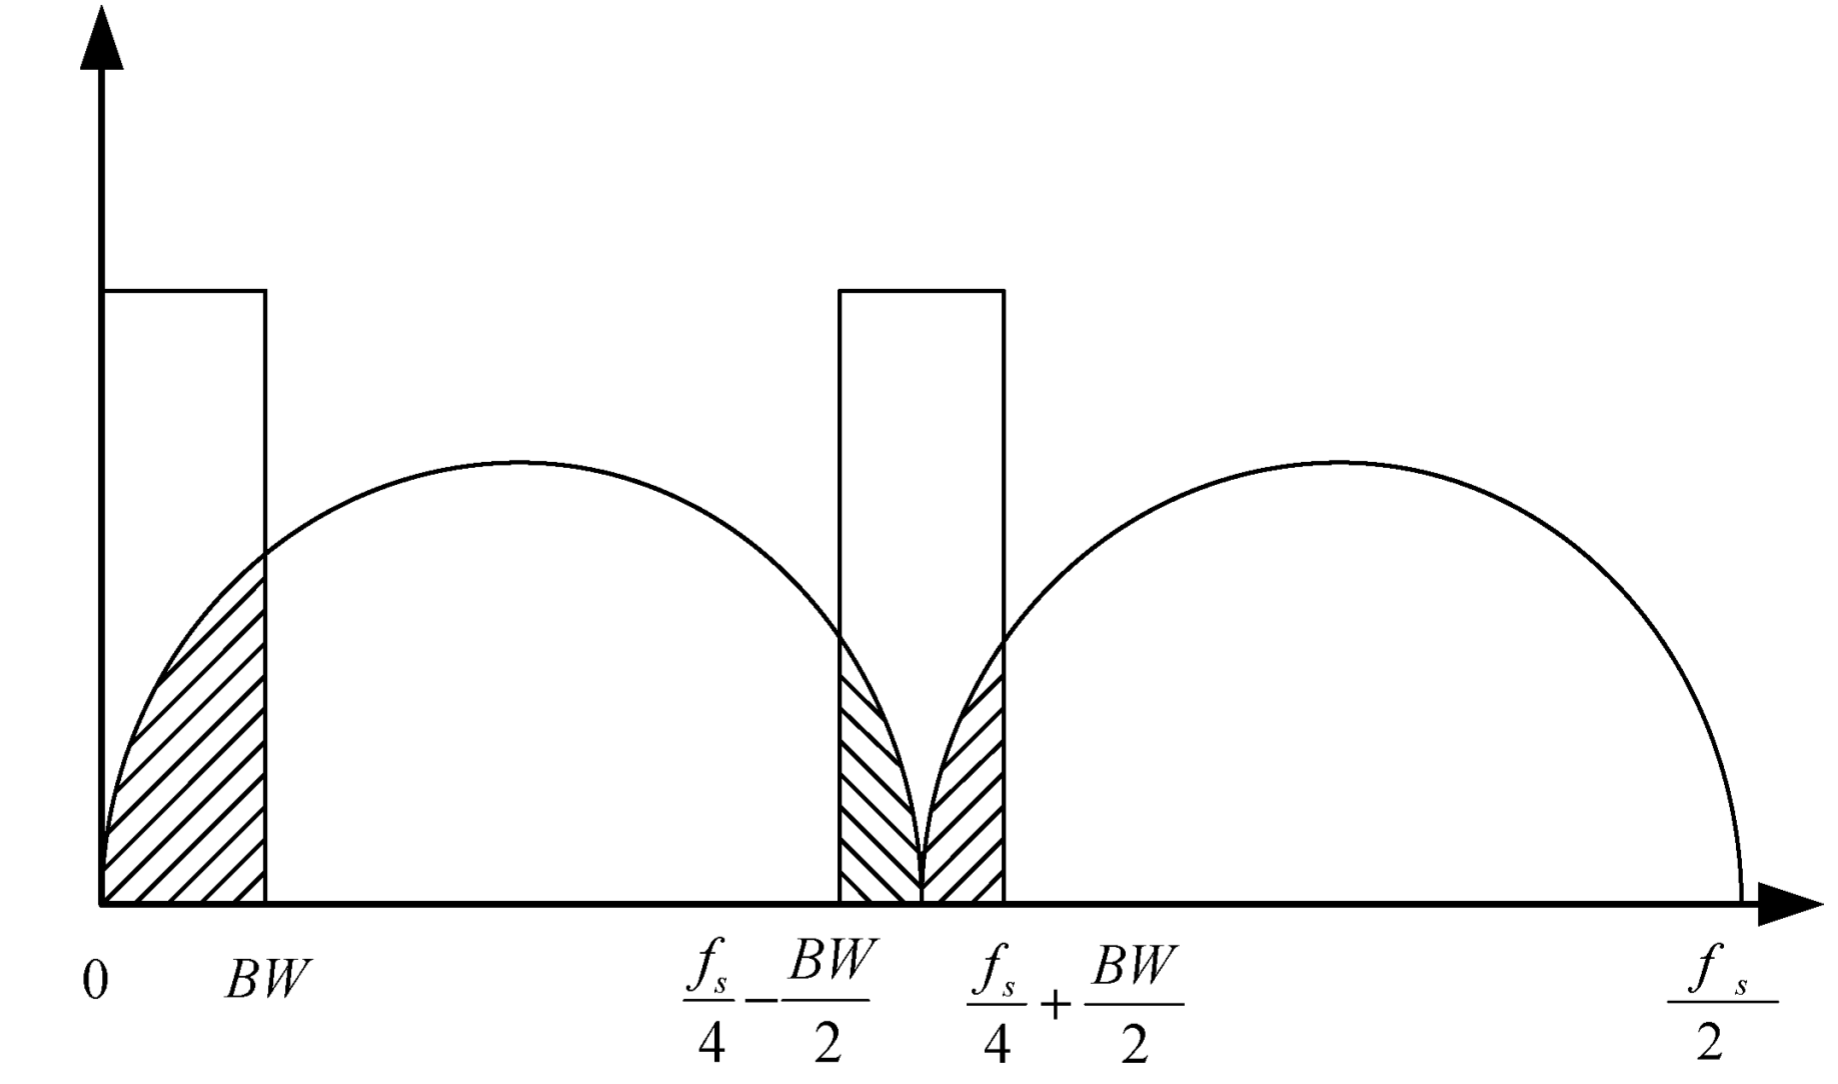
\includegraphics[scale=0.3]{./figs/Bwplot.png}
\end{figure}
\vspace{-0.5cm}
\begin{itemize}
	\item At $\omega = 0 or \pi$,
	\vspace{-0.5cm}
	\begin{equation*}
		SQNR = 6.02ENOB - 3.41 + 30log(OSR)dB
	\end{equation*}
	\vspace{-1cm}
	\item At intermediate zeroes,
	\vspace{-0.6cm}
	\begin{equation*}
		SQNR = 6.02ENOB - 3.41 + 6.02 + 30log(OSR)dB
	\end{equation*}
	\vspace{-1.3cm}
\end{itemize}
	Increase of 6.02dB is equivalent to increase in 1-bit precision of ADC!!
\end{frame}

\begin{frame}{Non-idealities}
	\begin{itemize}
		\item DC offset
		\item Gain mismatch
		\item Clock Jitter/Skew
		\item Bandwidth mismatch
		\item Non-linearity in VCO
	\end{itemize}
\end{frame}

\begin{frame}{DC offset}
\begin{figure}
	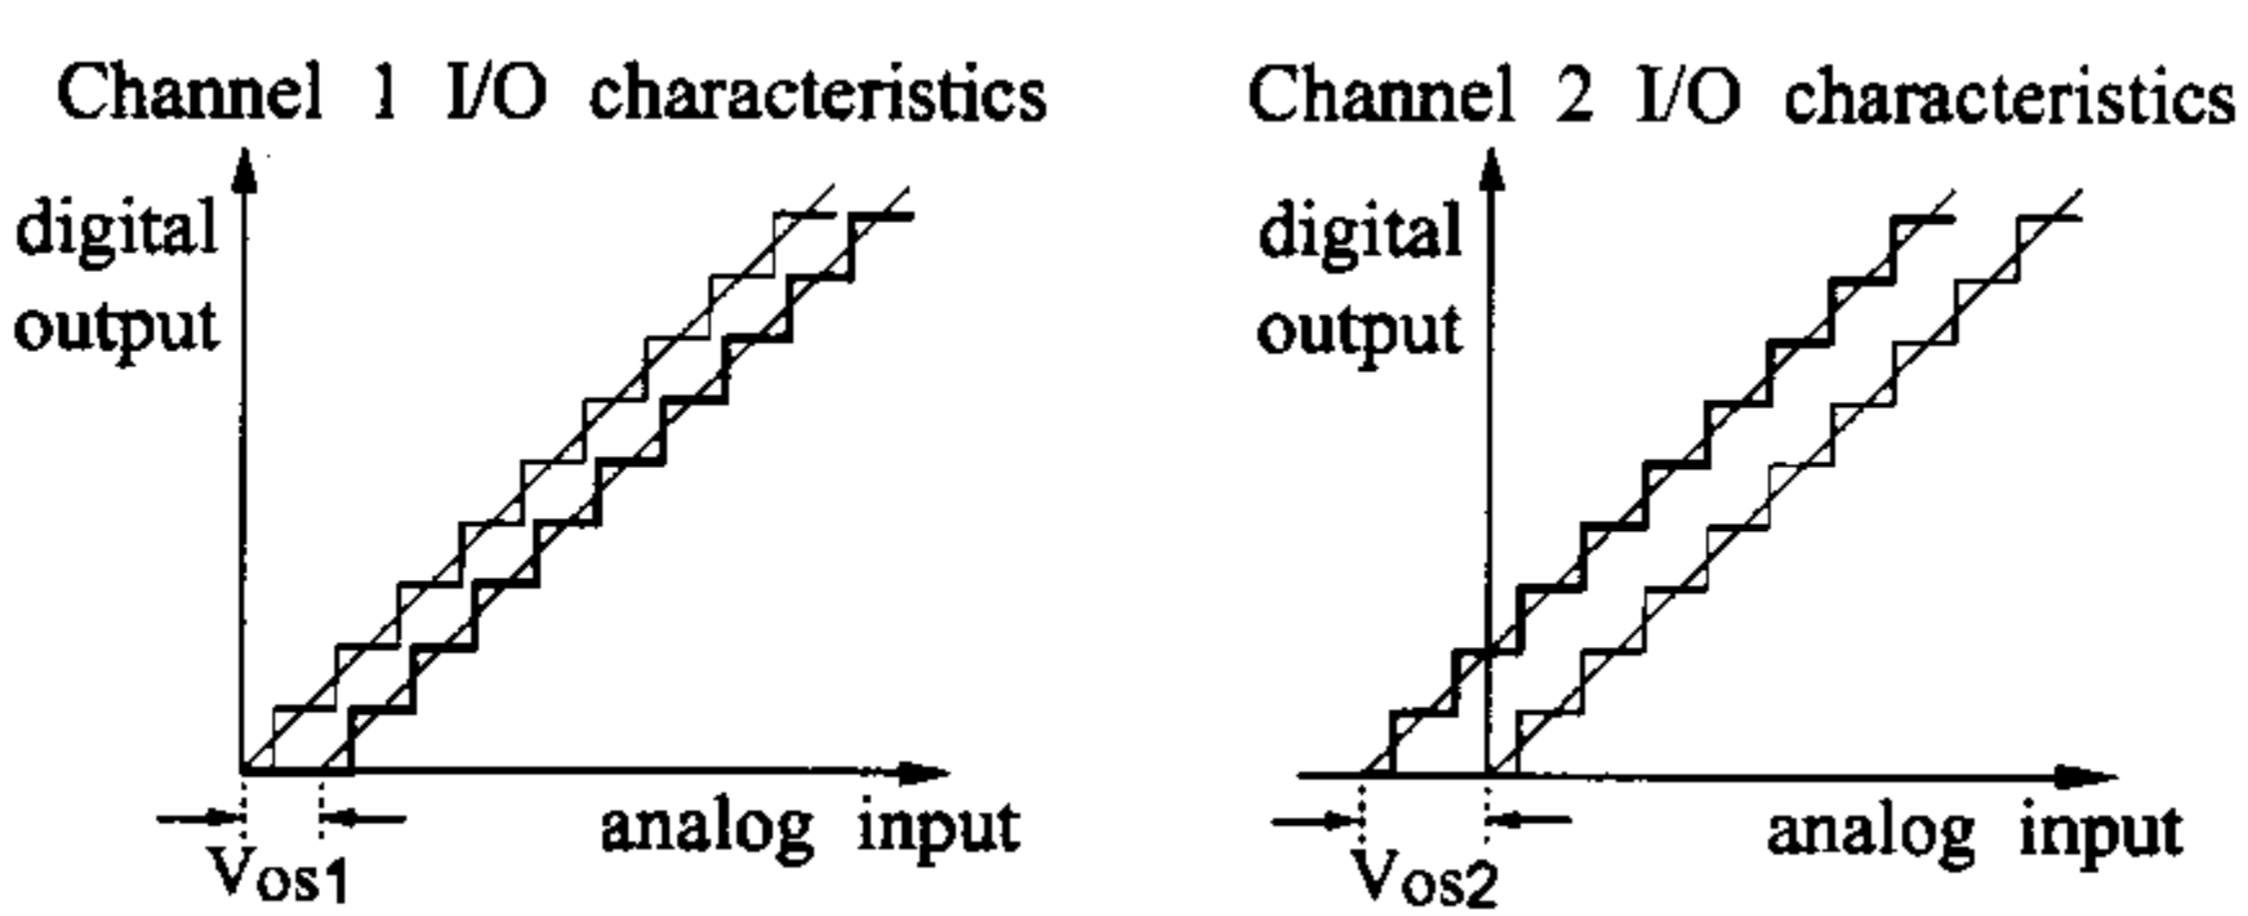
\includegraphics[scale=0.2]{./figs/Dc.png}
	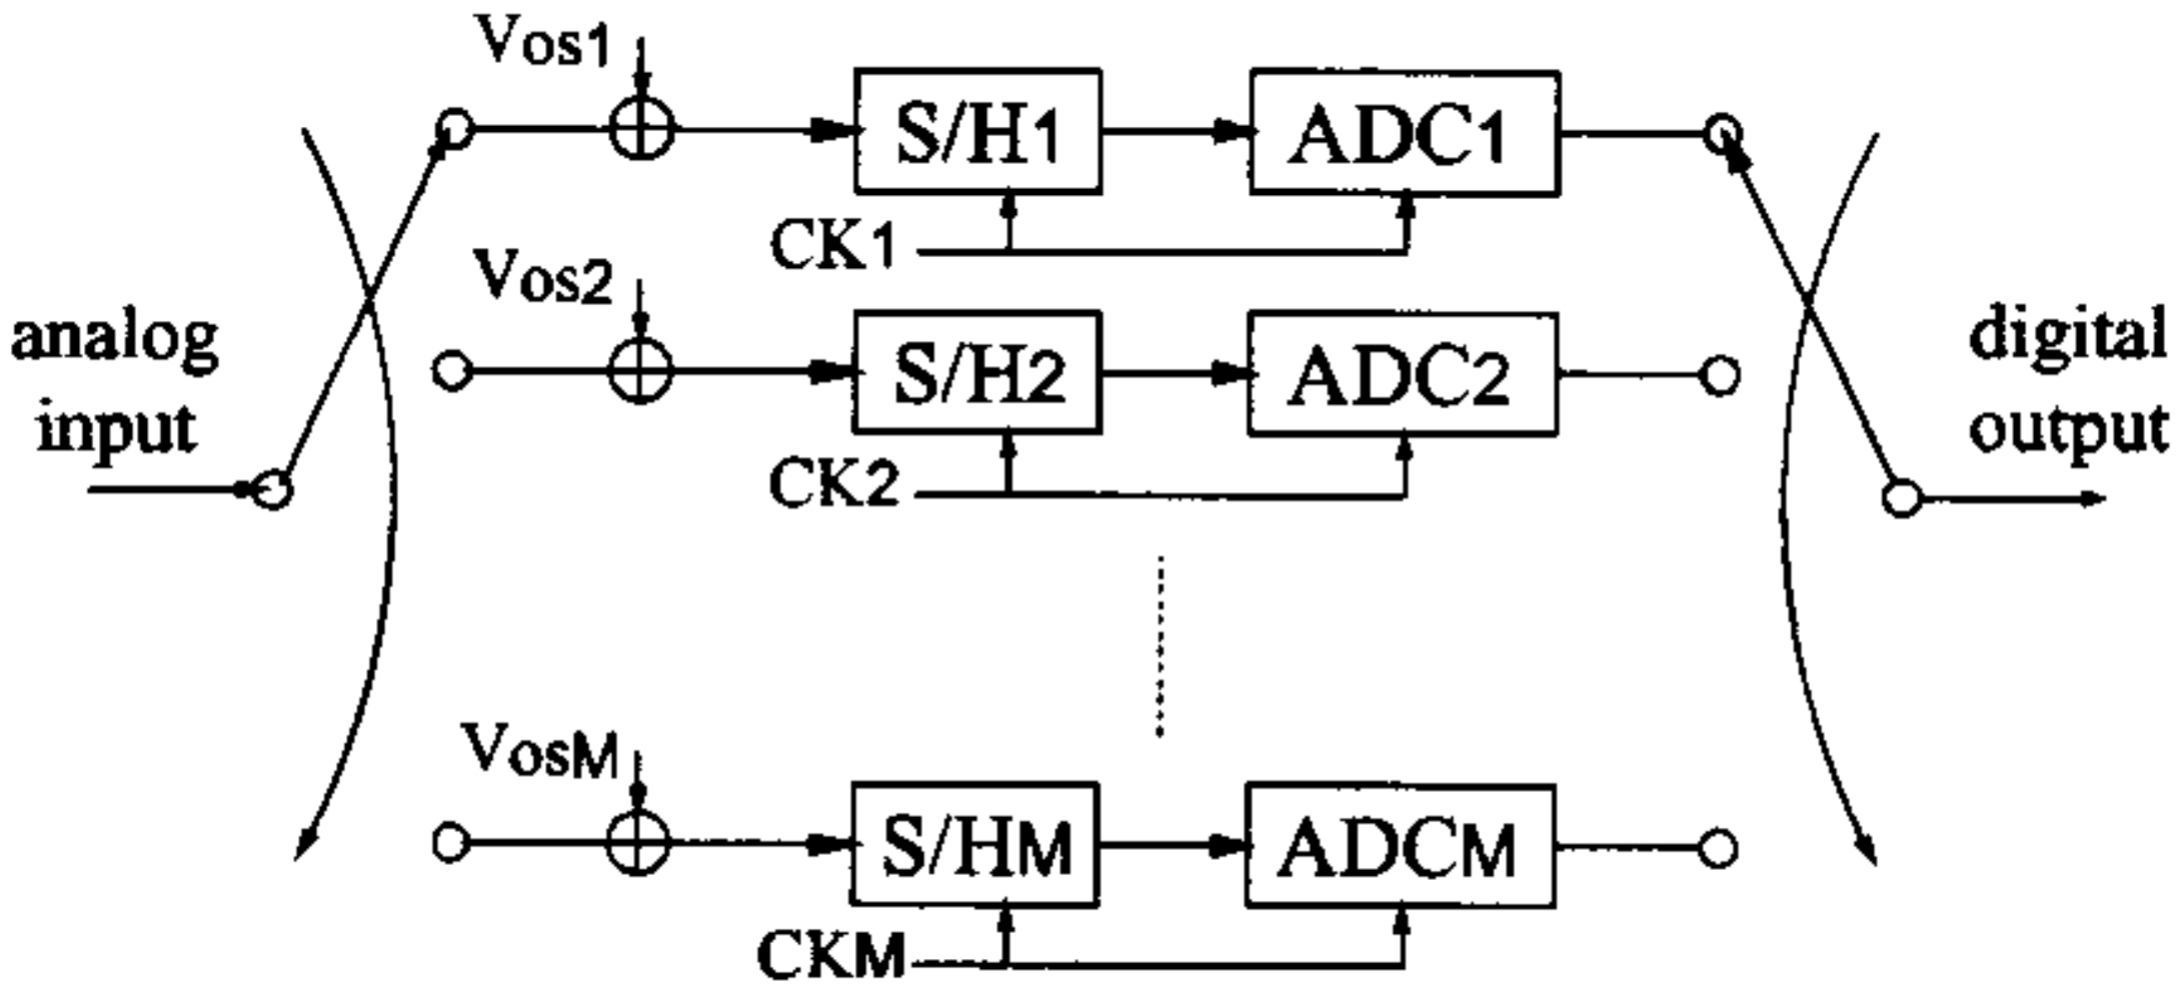
\includegraphics[scale=0.2]{./figs/Dccir.png}
\end{figure}
\end{frame}

\begin{frame}{DC offset}
\begin{figure}
	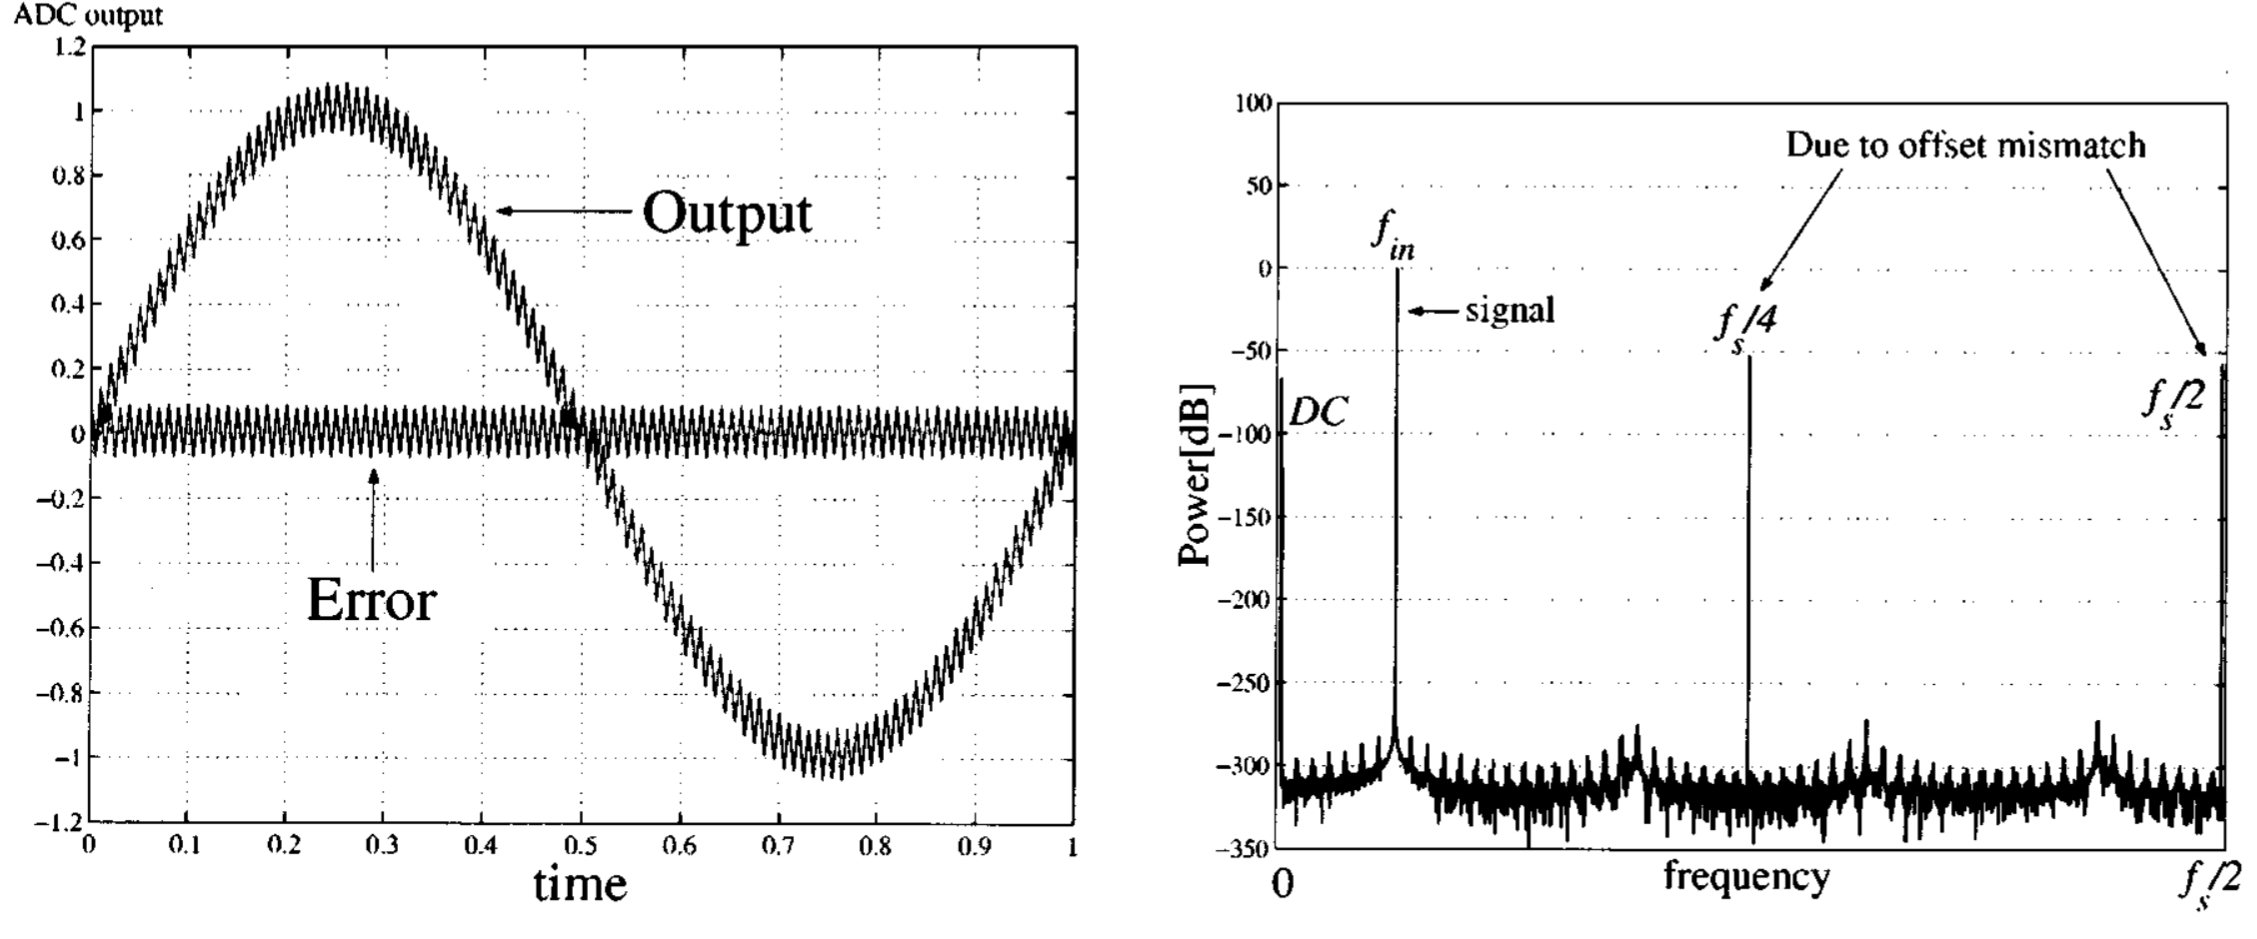
\includegraphics[scale=0.3]{./figs/Dcplot .png}
\end{figure}
\pause
\begin{itemize}
\item We can see that dc offset periodicity $\implies$ peaks at $\frac{k}{M}f_{s}$
\end{itemize}
\end{frame}

\begin{frame}{Gain mismatch}
\begin{figure}
	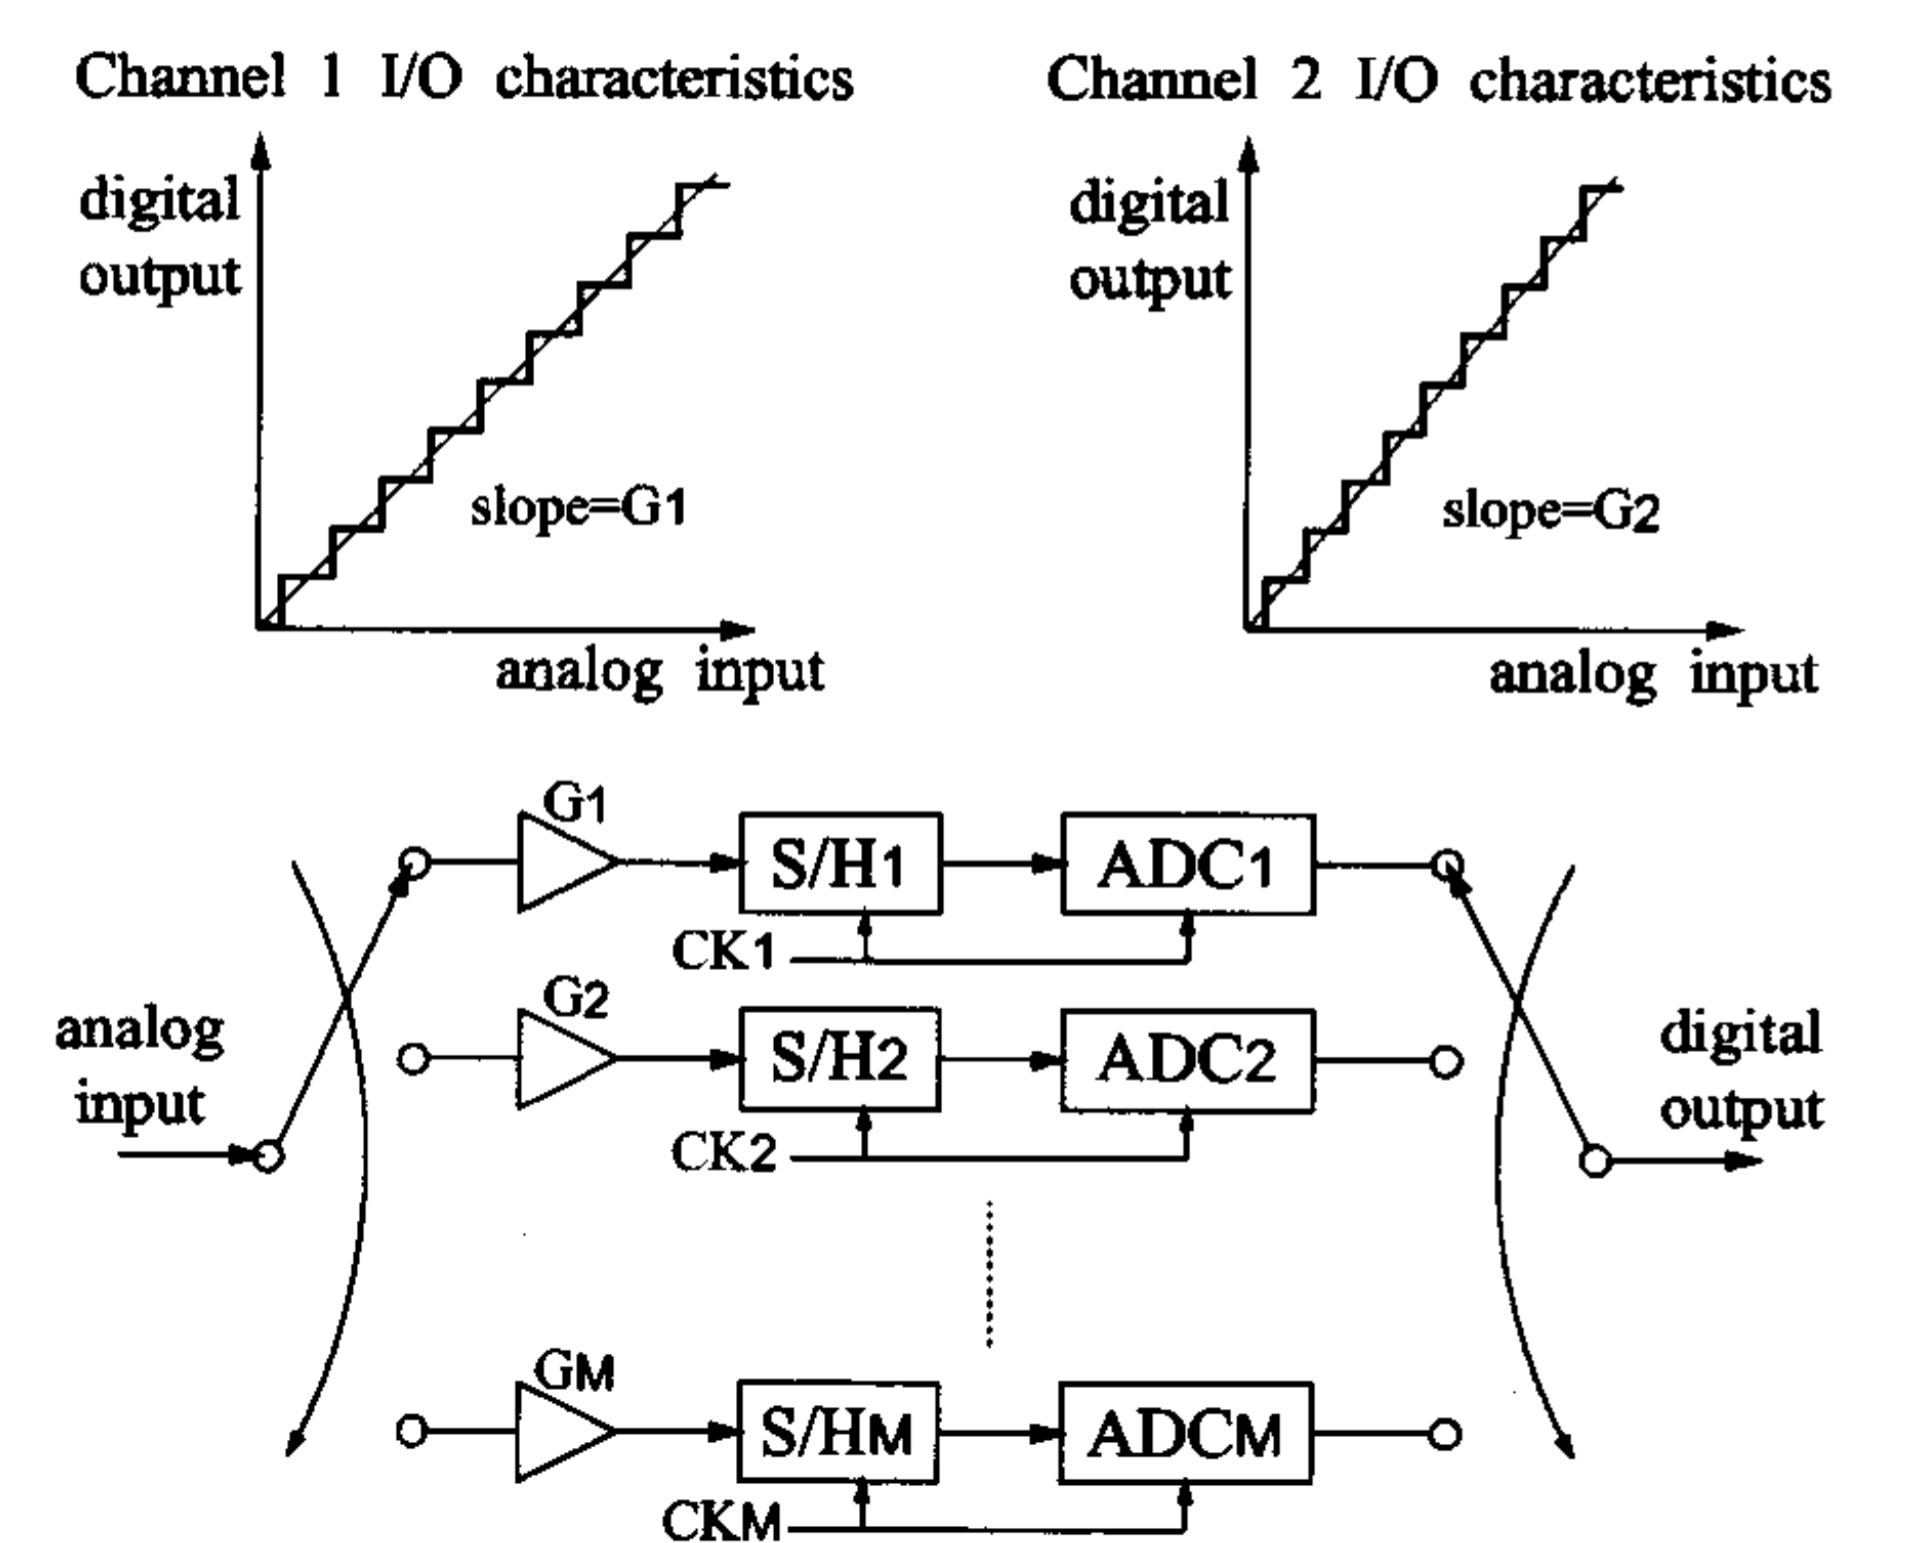
\includegraphics[scale=0.2]{./figs/Gain.png}
\end{figure}
\end{frame}

\begin{frame}{Gain mismatch}
\begin{figure}
	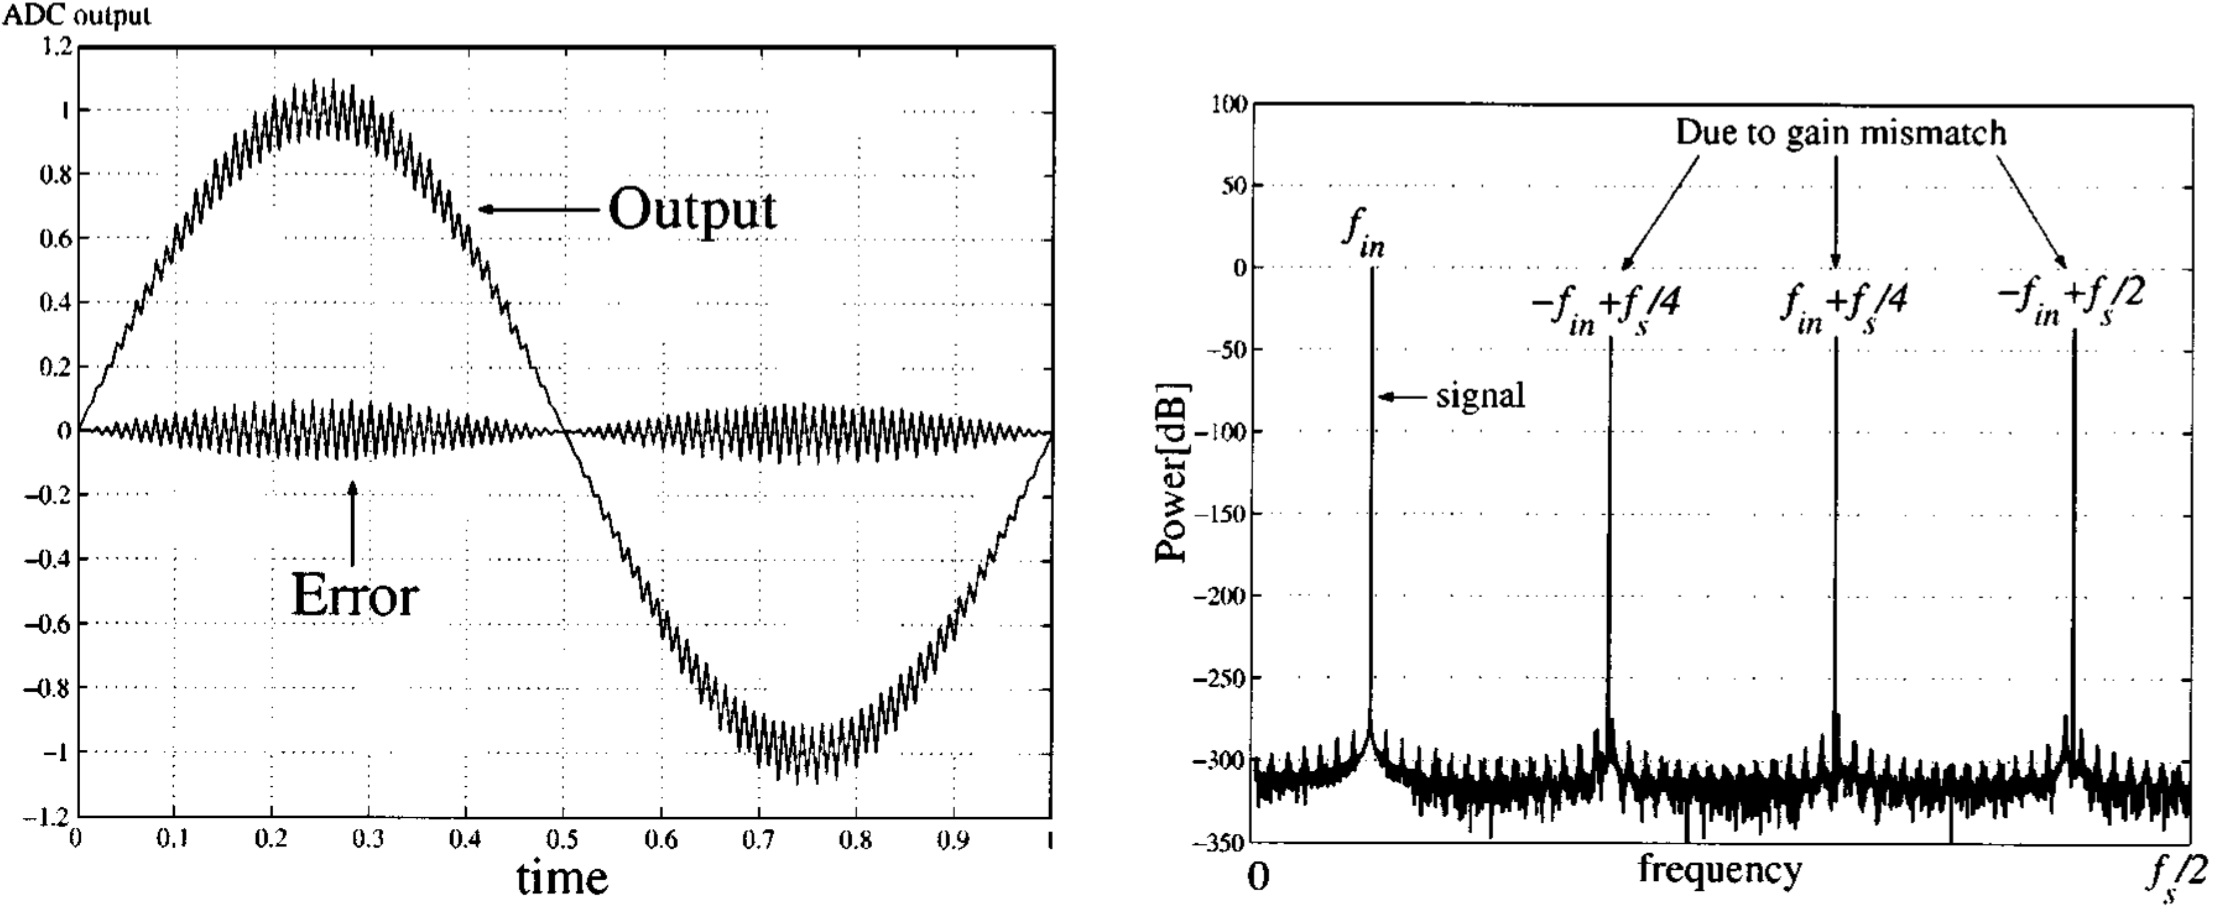
\includegraphics[scale=0.3]{./figs/Gainplot.png}
\end{figure}
\pause
\begin{itemize}
\item Gain mismatch can be looked as A.M $\implies$ peaks at $\pm f_{in} + \frac{k}{M}f_{s}$
\item Error at higher amplitude is more.
\end{itemize}
\end{frame}

\begin{frame}{Clock jitter}
\begin{figure}
	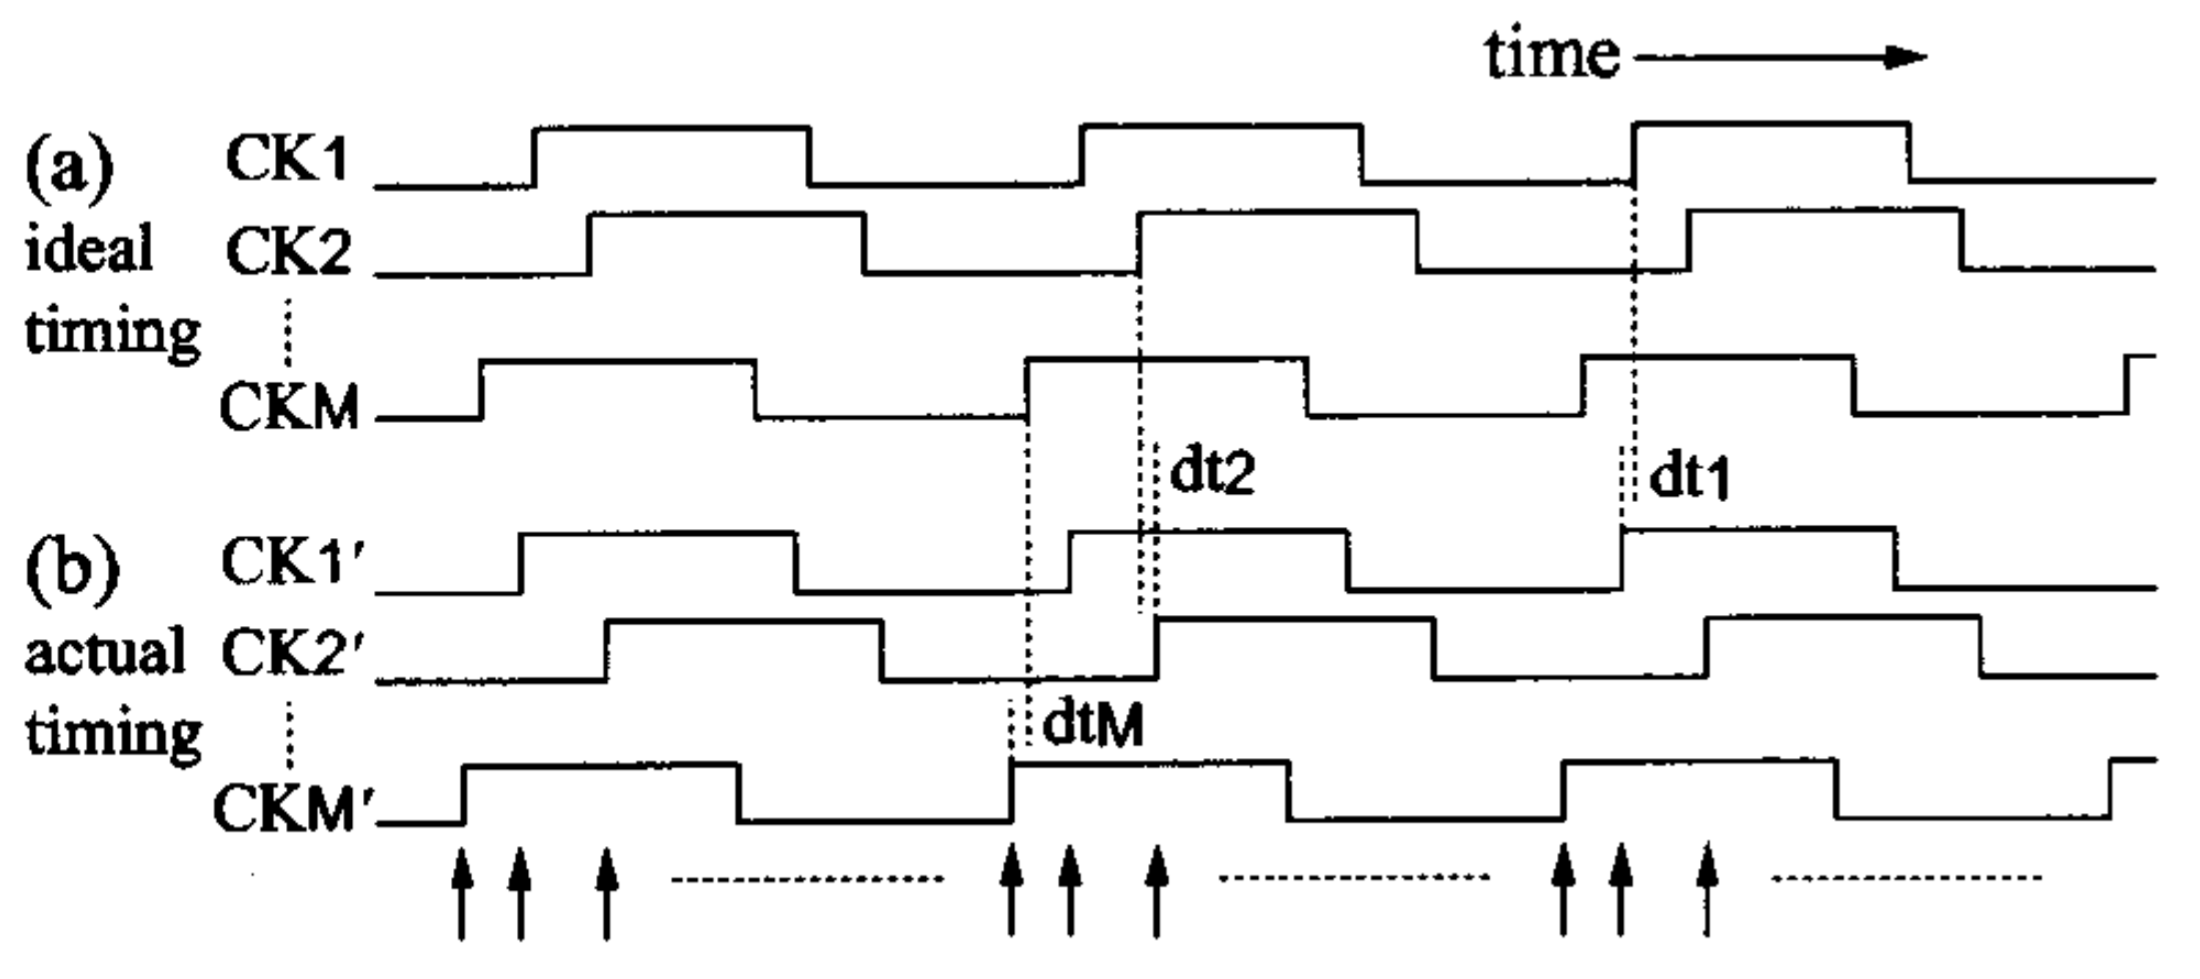
\includegraphics[scale=0.2]{./figs/Skew.png}
	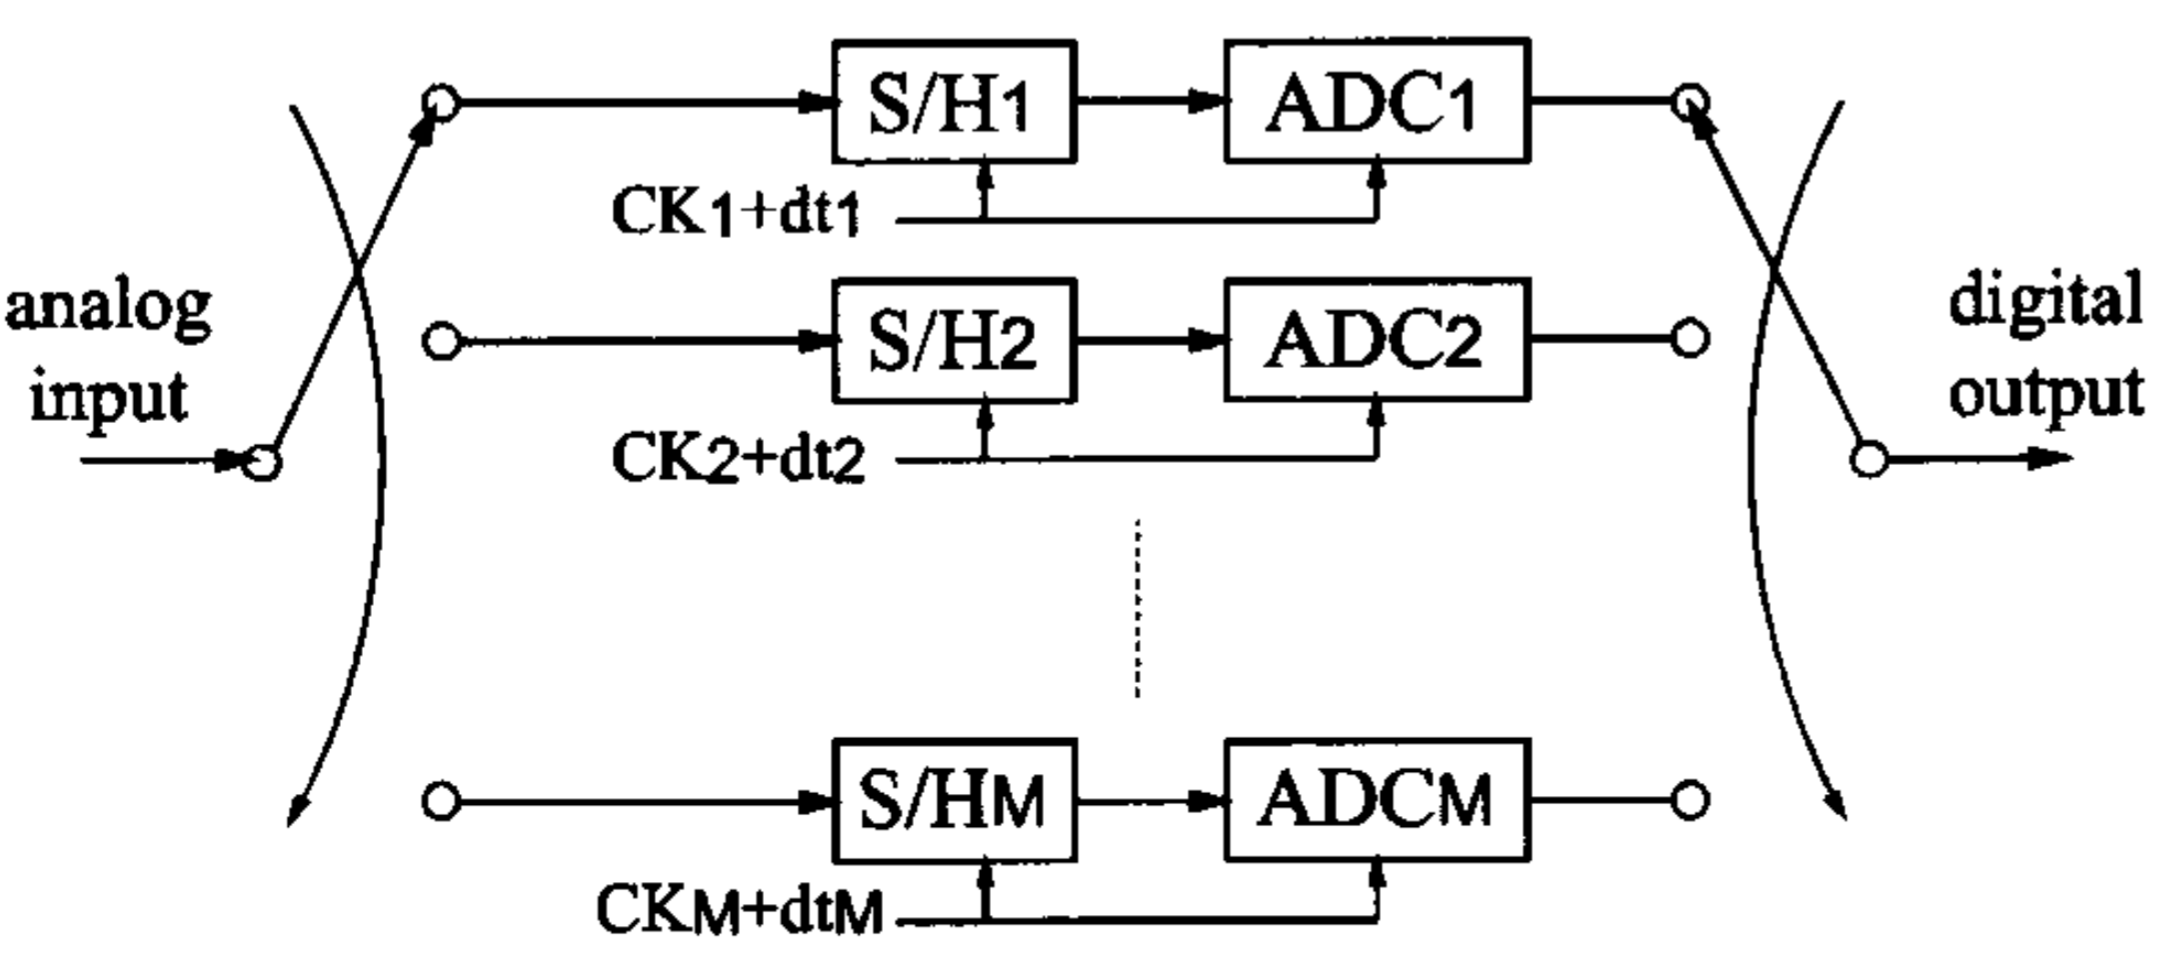
\includegraphics[scale=0.2]{./figs/Skewcir.png}
\end{figure}
\end{frame}

\begin{frame}{Clock jitter}
\begin{figure}
	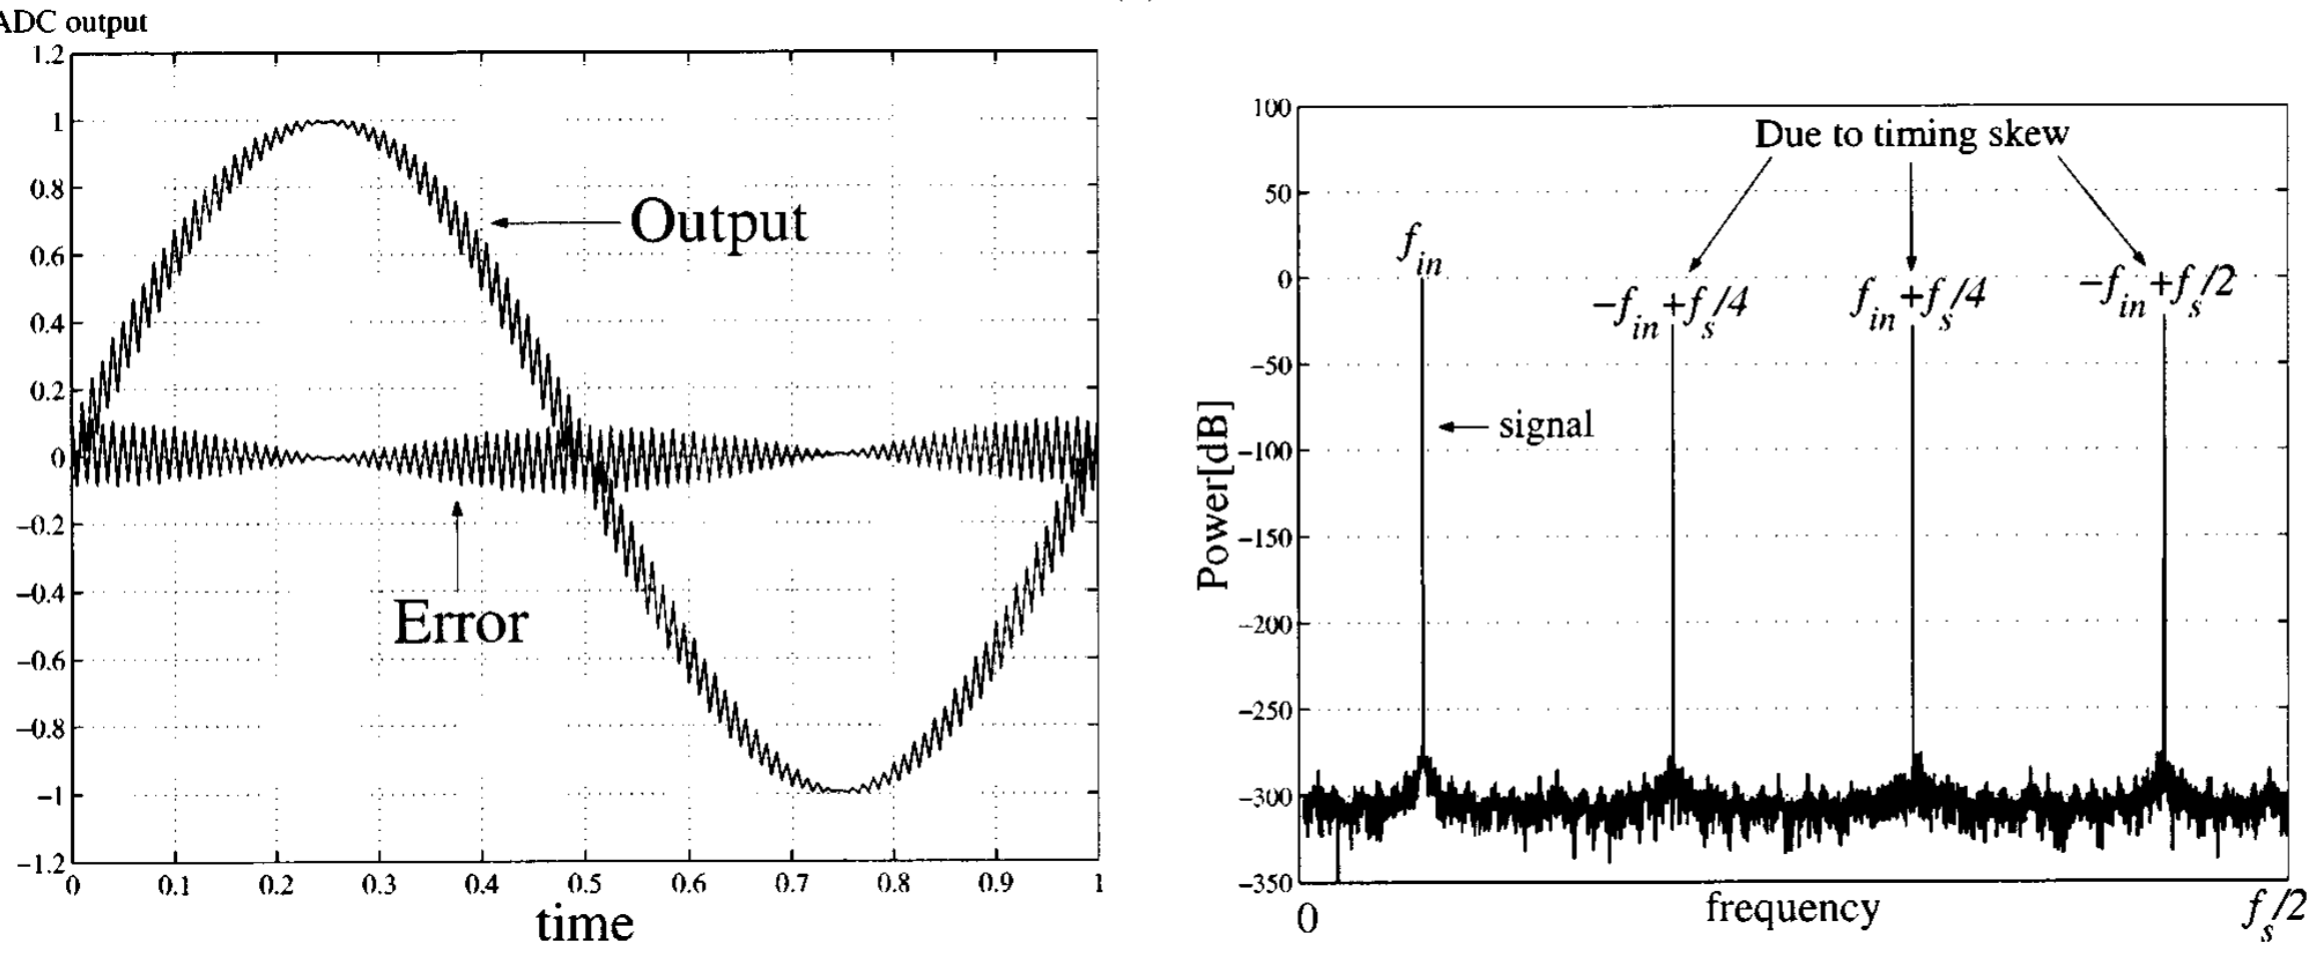
\includegraphics[scale=0.3]{./figs/Skewplot.png}
\end{figure}
\pause
\begin{itemize}
\item Clock skew behaves like P.M $\implies$ peaks at $\pm f_{in} + \frac{k}{M}f_{s}$.
\item Error is high at places where slew rate is more.
\end{itemize}
\end{frame}

\begin{frame}{SNR comparisions}
\begin{figure}
	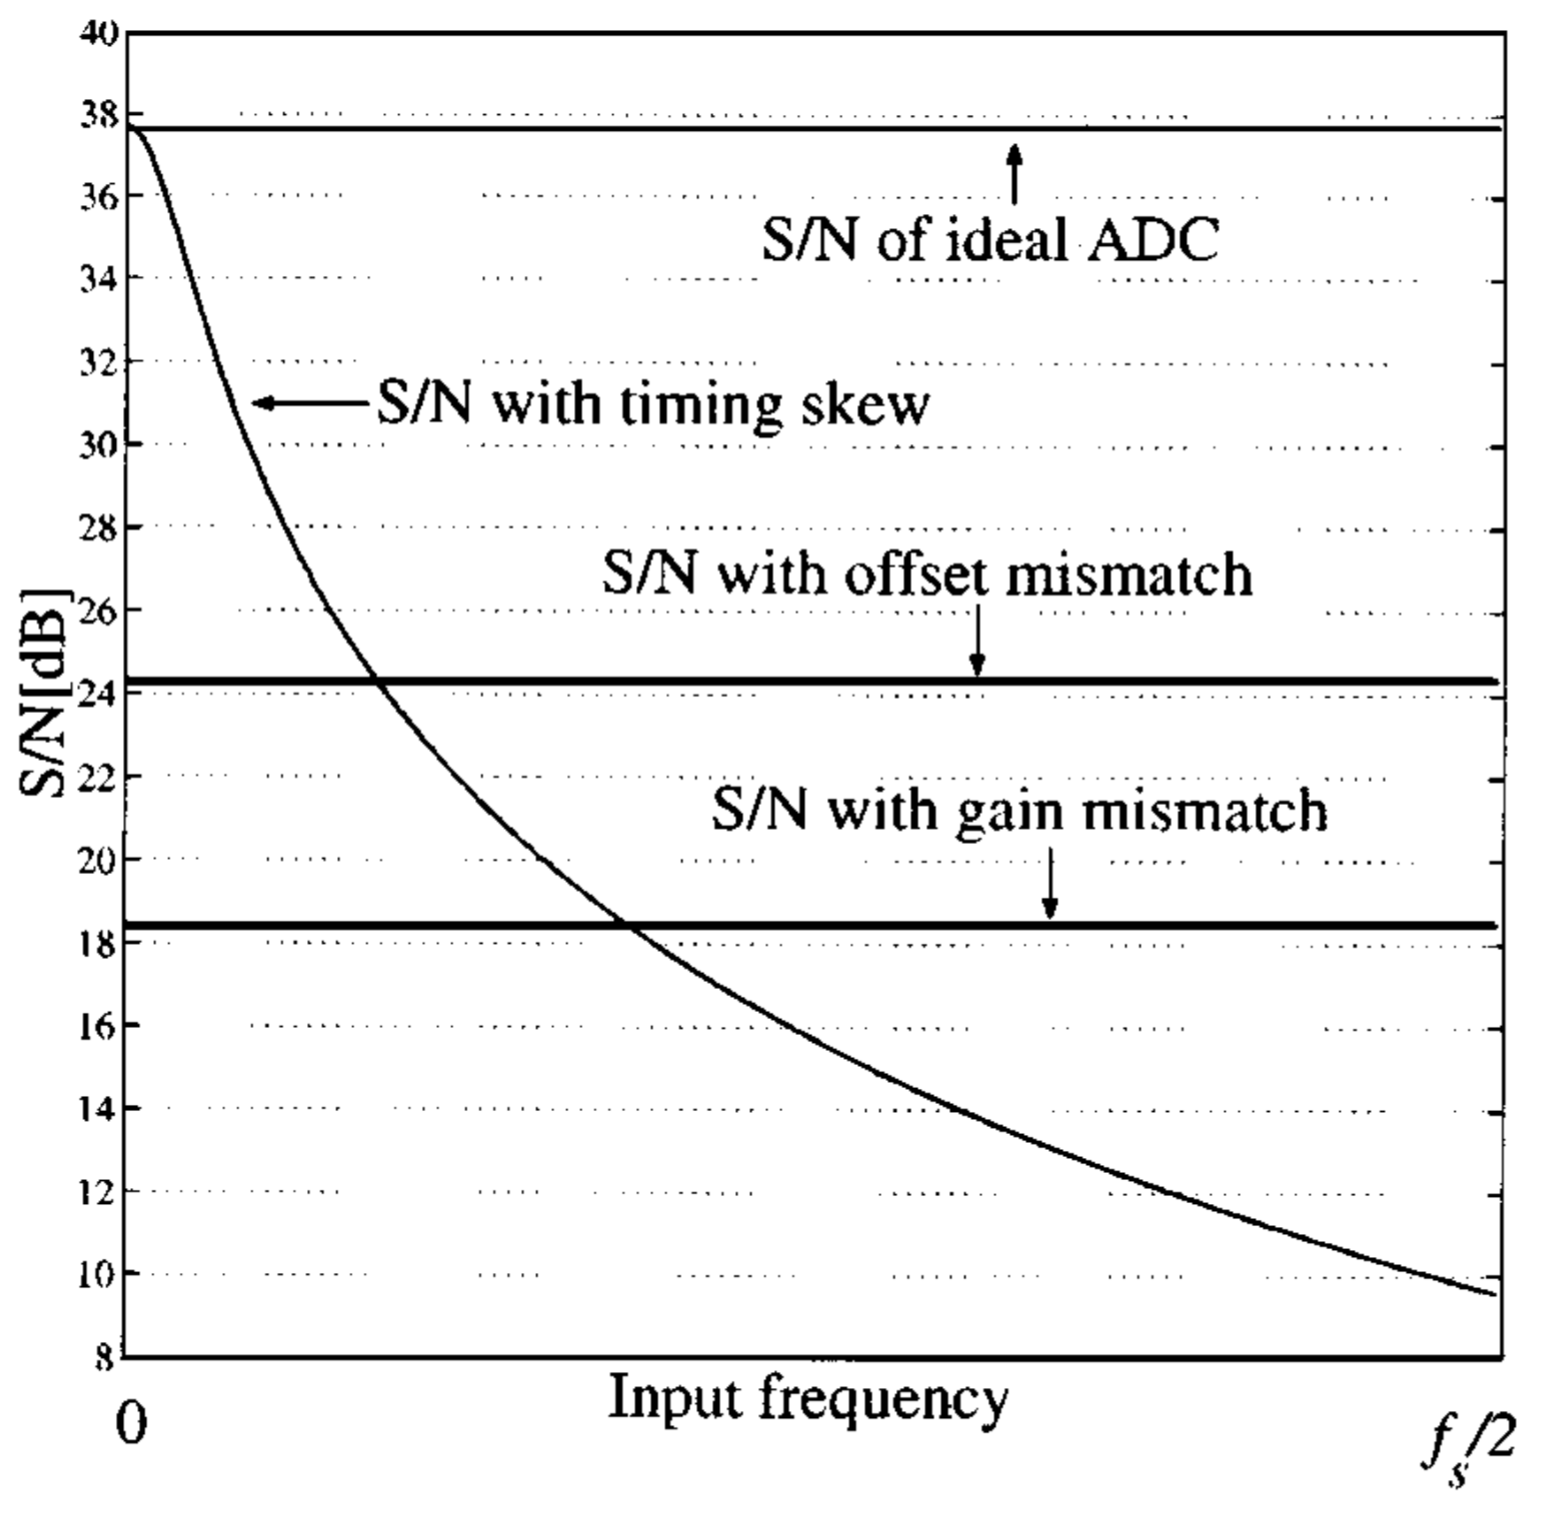
\includegraphics[scale=0.25]{./figs/Over.png}
\end{figure}
\end{frame}

\begin{frame}{}
\centering
 \Huge
 Thank You
\end{frame}
\end{document}